\documentclass[conference]{IEEEtran}
\usepackage[T1]{fontenc}
\usepackage{amsmath,amssymb}
\let\proof\relax
\let\endproof\relax
\usepackage{amsthm}
\usepackage{graphicx}
\usepackage{booktabs}
\usepackage{array}
\usepackage{multirow}
\usepackage{algorithm}
\usepackage{algpseudocode}
\usepackage{xcolor}
\usepackage{tikz}
\usetikzlibrary{arrows.meta,positioning,fit}
\usepackage{pgfplots}
\pgfplotsset{compat=1.18}
\usepackage[hidelinks]{hyperref}
\newcommand{\ket}[1]{\lvert #1 \rangle}
\newcommand{\bra}[1]{\langle #1 \rvert}
\newcommand{\Fk}{\mathcal{F}_k}
\newcommand{\Ak}{A_k}
\newcommand{\Otau}{O_\tau}
\newcommand{\Ptau}{P_\tau}
\newcommand{\Fstar}{F^{*}}
\newcommand{\bigO}{\mathcal{O}}
\newcommand{\poly}{\operatorname{poly}}
\newtheorem{definition}{Definition}
\newtheorem{proposition}{Proposition}
\newtheorem{lemma}{Lemma}
\theoremstyle{remark}
\newtheorem{remark}{Remark}
\definecolor{qaccent}{HTML}{1F4E79}
\definecolor{qgray}{gray}{0.55}


\title{Quantum Minimum Finding for Cardinality-Constrained Maximum Flow Interdiction}
\author{\IEEEauthorblockN{Vinicius Testa Passos}
\IEEEauthorblockA{Inteli -- Instituto de Tecnologia\\
e Liderança\\
S\~ao Paulo, Brazil\\
vinicius.passos@sou.inteli.edu.br}
\and
\IEEEauthorblockN{Erinaldo Fonseca}
\IEEEauthorblockA{Advisor\\
Inteli -- Instituto de Tecnologia\\
e Liderança\\
S\~ao Paulo, Brazil}
\and
\IEEEauthorblockN{Bryan Kano}
\IEEEauthorblockA{Advisor\\
Inteli -- Instituto de Tecnologia\\
e Liderança\\
S\~ao Paulo, Brazil}}

\begin{document}
\maketitle
\begin{abstract}
The maximum flow network interdiction problem (MFNIP) asks which arcs of a capacitated network an interdictor with a limited budget should remove to minimize the maximum flow that remains. It models how the loss of critical routes reduces the capacity of a supply chain. We propose a quantum interface that applies the quantum minimum-finding algorithm of Dürr and Høyer to the cardinality-constrained MFNIP. The interface assigns one qubit to each arc, prepares a superposition of Dicke states so that the search covers only the $N$ feasible interdiction plans, and uses a phase oracle that compares the follower's maximum flow with a threshold. We prove that, with this interface, the algorithm finds an optimal plan with probability at least one half using $\mathcal{O}(\sqrt{N})$ applications of polynomial-size circuits, whereas any classical algorithm that only evaluates the flow of candidate plans needs $\Omega(N)$ evaluations. In a query-level simulation on 30 layered networks with 9 to 974{,}121 feasible plans, the mean cost of minimum finding grew as $N^{0.494}$ (95\% confidence interval $[0.460,0.523]$) and that of a classical random-order search as $N^{0.975}$, and every run found the optimum within the bound of the proof. We also report qubit and gate counts of the state preparation and of an arithmetic oracle for networks with up to 14 arcs. On the IBM Heron processor \texttt{ibm\_fez}, amplitude amplification for a three-arc network returned the optimal plan in 81.5\% of the shots, against 25\% under uniform sampling. The speedup is quadratic, asymptotic, and relative to exhaustive search over the feasible plans. On every instance we tested, a mixed-integer programming solver was faster by several orders of magnitude.
\end{abstract}

\begin{IEEEkeywords}
network interdiction, maximum flow, Grover search, quantum minimum finding, Dicke states, query complexity
\end{IEEEkeywords}

\section{Introduction}\label{sec:intro}

Strikes, natural disasters, armed conflicts, and the closure of a port, bridge, or strait can cut critical routes of a supply chain and sharply reduce the amount of goods a logistics network can deliver~\cite{supplychain_resilience}. Identifying the routes whose loss costs the most capacity tells planners where to invest in protection and redundancy. Operations research models this question as the \emph{maximum flow network interdiction problem} (MFNIP)~\cite{wood1993,smith2020}. The network has a source, a sink, and a capacity on each arc. An interdictor with a limited budget removes arcs, and a network user, the follower, then sends as much flow as possible from the source to the sink through the remaining arcs. The interdictor seeks the removal plan that minimizes this maximum flow. The problem is bilevel because evaluating even a single plan requires solving an optimization problem, namely the follower's maximum flow. A maximum flow can be computed in polynomial time, but the general problem of choosing the best plan is NP-hard~\cite{wood1993}. Figure~\ref{fig:example} in Section~\ref{sec:method} shows a small instance.

This paper asks what quantum computers can offer for a problem of this kind, and three facts constrain the answer. First, exact classical methods perform well in practice. Wood~\cite{wood1993} reformulated the MFNIP as a single-level mixed-integer linear program (MILP) by replacing the follower's maximum flow with the equivalent minimum cut (Section~\ref{sec:bg-mfnip}). In our scaling study, a modern MILP solver certified optimal plans for networks with thousands of nodes within 20 seconds (Section~\ref{sec:results-classical}), whereas the networks that fit on current quantum devices have a few dozen arcs and are trivial for classical solvers. Second, current quantum processors belong to the noisy intermediate-scale quantum (NISQ) era~\cite{preskill2018}. They have few qubits, limited connectivity, and noise, so they can only run shallow circuits. Third, the quantum optimizers most often applied to combinatorial problems, quantum annealing~\cite{kadowaki1998} and the quantum approximate optimization algorithm (QAOA)~\cite{farhi2014}, require a quadratic unconstrained binary optimization (QUBO) model~\cite{lucas2014,glover2019}. For the MFNIP, such a model must encode the node partition, the cut, and the budget as penalty terms, with slack variables for the inequalities. This encoding adds qubits, lets the device return infeasible plans, and comes with no performance guarantee. A quantum method for the MFNIP should therefore not be presented as a competitor of the MILP at the current scale. What it can offer is a provable speedup over a well-defined classical reference, together with an honest account of its cost in quantum resources.

The question that guides this work is \emph{what speedup a quantum search algorithm can provably achieve over classical exhaustive search for the MFNIP, at what cost in qubits and gates, and how it compares with the classical method used in practice.} Our objective is to design, analyze, and verify a quantum interface that applies the quantum minimum-finding algorithm of Dürr and Høyer~\cite{durr1996}, a Grover-type method~\cite{grover1996,bbht1998}, to the MFNIP without losing its quadratic speedup. The quadratic speedup of Grover search over brute force is well known, but applying it to a bilevel problem raises two difficulties. The oracle must compute the follower's maximum flow for every plan in superposition, and the budget must be enforced without enlarging the search space.

The work proceeds in six steps. We (i) restrict the problem to its cardinality variant, in which every arc costs one unit and at most $k$ arcs are removed, and compare the number $N$ of feasible plans with the size of the hypercube; (ii) design the quantum interface, which comprises the encoding, a state preparation that enforces the budget, a threshold predicate on the maximum flow, and the corresponding phase oracle; (iii) prove the query complexity of minimum finding with this interface and show that it is optimal; (iv) generate instances of increasing size with fixed seeds and validate each simulator against an exact reference; (v) measure in simulation how the cost of finding the optimum grows with $N$ for the quantum algorithm and for classical rivals, using the MILP both as the reference optimum and as the practical baseline; and (vi) count the qubits and gates of the interface as functions of the network size and run amplitude amplification on an IBM quantum processor.

We state two refutable hypotheses, fixed before the experiments (Section~\ref{sec:method-hypotheses}). Success always means finding an exactly optimal plan certified by the MILP. Hypothesis H1 concerns simulation. On 30 layered networks with 6 to 27 nodes, 8 to 70 arcs, and $N$ between 9 and 974{,}121, the mean cost of minimum finding until an optimal plan is first measured grows as $N^{\beta}$ with $\beta\in[0.4,0.6]$, whereas a classical random-order search grows with an exponent close to one. Because our simulator samples from the exact amplification probabilities, H1 checks the correctness of the implementation rather than the behavior of a physical oracle. Hypothesis H2 concerns hardware. On an IBM processor and for a network with three nodes and three arcs ($k=1$, $N=4$), the frequency of the optimal plan after the optimal number of Grover iterations is significantly greater than the uniform baseline $1/N$ (one-sided binomial test at level $0.05$). Since this baseline is weak, we also compare the hardware frequencies with the theoretical probabilities and with a noisy simulator in an exploratory analysis.

\paragraph{Contributions} This paper makes four contributions.
\begin{enumerate}
\item[C1.] A \emph{quantum interface} for the MFNIP (Section~\ref{sec:interface}). It uses one qubit per arc and a state preparation based on Dicke states~\cite{bartschi2019} that enforces the cardinality budget, so that the search covers exactly the $N=\sum_{i\le k}\binom{m}{i}$ feasible plans. A threshold predicate on the maximum flow, its phase oracle, and a classical threshold loop complete the interface.
\item[C2.] A \emph{provable speedup} (Proposition~\ref{prop:advantage} in Section~\ref{sec:advantage}). With $\bigO(\sqrt{N})$ applications of polynomial-size circuits, the algorithm finds an optimal plan with probability at least $1/2$, whereas any classical algorithm that only evaluates candidate plans needs $\Omega(N)$ flow evaluations. The bound is optimal in the query model.
\item[C3.] A \emph{verification} of the interface (Section~\ref{sec:results}). It comprises the growth of the cost to the optimum in a query-level simulation, the qubit and gate counts of the state preparation and of an arithmetic oracle, and the amplification of the optimal plan on ideal and noisy simulators and on an IBM quantum processor.
\item[C4.] A \emph{delimitation} of the speedup (Sections~\ref{sec:advantage} and~\ref{sec:discussion}). The speedup is quadratic, asymptotic, and relative to exhaustive search over the feasible plans, and on every instance we studied the MILP is orders of magnitude faster than both searches.
\end{enumerate}
A systematic literature search (Section~\ref{sec:rel-novelty}) found quantum approaches to other interdiction problems~\cite{peddireddy2026,sutcliffe2026}, but none for the MFNIP and none in which the state preparation enforces the interdiction budget.

\paragraph{Organization} Section~\ref{sec:background} reviews the background and Section~\ref{sec:related} the related work. Section~\ref{sec:interface} presents the interface, and Section~\ref{sec:advantage} proves the speedup. Section~\ref{sec:method} describes the experiments, and Section~\ref{sec:results} reports the results. Section~\ref{sec:discussion} discusses the results and their limitations, and Section~\ref{sec:conclusion} concludes.

\section{Background}\label{sec:background}

This section fixes the notation and collects the classical and quantum results used by the interface of Section~\ref{sec:interface} and by the analysis of Section~\ref{sec:advantage}.

\subsection{Maximum flow and minimum cut}\label{sec:bg-flow}

Let $G=(V,A)$ be a directed network with $n=|V|$ nodes, $m=|A|$ arcs, a source $s$, a sink $t\neq s$, and integer capacities $u_a>0$ for $a\in A$. For a node $v$, let $\delta^{+}(v)$ and $\delta^{-}(v)$ be the sets of arcs that leave and enter $v$. An \emph{$s$--$t$ flow} is a vector $f\in\mathbb{R}^{m}$ that satisfies the capacity constraints $0\le f_a\le u_a$ for all $a\in A$ and the conservation constraints
\begin{equation}\label{eq:conservation}
  \sum_{a\in\delta^{-}(v)} f_a \;=\; \sum_{a\in\delta^{+}(v)} f_a \qquad \text{for all } v\in V\setminus\{s,t\}.
\end{equation}
The value of the flow, $|f|=\sum_{a\in\delta^{+}(s)}f_a-\sum_{a\in\delta^{-}(s)}f_a$, is the net amount that leaves the source, and the maximum flow problem asks for a flow of maximum value. An \emph{$s$--$t$ cut} is a set of nodes $S\subset V$ with $s\in S$ and $t\notin S$, and its capacity is the sum of the capacities of the arcs that leave $S$. The max-flow min-cut theorem of Ford and Fulkerson~\cite{fordfulkerson1956} states that the maximum value of an $s$--$t$ flow equals the minimum capacity of an $s$--$t$ cut. The maximum flow problem can be solved in polynomial time~\cite{ahuja1993}.

Throughout the paper, an \emph{interdiction vector} $x\in\{0,1\}^{m}$ indicates the removed arcs ($x_a=1$ means that arc $a$ is interdicted), and
\begin{equation}\label{eq:F}
  \begin{aligned}
  F(x) = \max\bigl\{\, |f| :{}& f \text{ satisfies \eqref{eq:conservation} and}\\
  & 0\le f_a\le u_a(1-x_a)\ \text{for all } a\in A \,\bigr\}
  \end{aligned}
\end{equation}
is the value of the maximum $s$--$t$ flow after the interdiction. Evaluating $F(x)$ costs one maximum flow computation, which is polynomial in $n$ and $m$. We write $|x|=\sum_{a}x_a$ for the number of interdicted arcs, which is the Hamming weight of $x$.

\subsection{The maximum flow network interdiction problem}\label{sec:bg-mfnip}

\paragraph{Bilevel formulation.} Each arc has an interdiction cost $c_a\in\mathbb{Z}_{>0}$, and the interdictor has a budget $B$. The MFNIP is a Stackelberg game in which the interdictor, the leader, first removes a set of arcs within the budget, and the network user, the follower, then sends a maximum flow through the remaining network~\cite{wood1993,smith2020}. The optimal value of the problem is
\begin{equation}\label{eq:mfnip}
  \Fstar \;=\; \min_{x\in\{0,1\}^{m}} \bigl\{\, F(x) \;:\; c^{\top}x\le B \,\bigr\},
\end{equation}
where the inner problem $F(x)$ of \eqref{eq:F} is the follower's linear program.

\paragraph{Single-level reformulation.} Because the follower's problem is a linear program, it can be replaced by its dual, the minimum cut problem, and the two minimizations merge into one. Wood~\cite{wood1993} linearized the product of the cut and interdiction variables and obtained a MILP with three groups of binary variables. The variable $\alpha_i$ gives the side of node $i$ in the cut ($\alpha_i=0$ on the source side and $\alpha_i=1$ on the sink side), $\gamma_a$ indicates that arc $a$ crosses the cut and is \emph{not} interdicted, so that its capacity counts toward the cut, and $x_a$ indicates that arc $a$ is interdicted. The model is
\begin{equation}\label{eq:milp}
\begin{aligned}
  \min_{\alpha,\gamma,x}\quad & \sum_{a\in A} u_a\gamma_a \\
  \text{s.t.}\quad & \alpha_i-\alpha_j+\gamma_a+x_a \ge 0,\quad a=(i,j)\in A,\\
  & \alpha_s=0,\qquad \alpha_t=1, \\
  & c^{\top}x\le B, \\
  & \alpha\in\{0,1\}^{n},\quad \gamma,x\in\{0,1\}^{m}.
\end{aligned}
\end{equation}

\paragraph{Complexity.} Wood~\cite{wood1993} proved by reduction from the clique problem that the decision version of the MFNIP is strongly NP-complete. According to Zenklusen~\cite{zenklusen2010}, the result holds even when every interdiction cost is $1$ or $\infty$, that is, with unit costs and some arcs that cannot be interdicted.

\paragraph{Cardinality variant.} This paper studies the variant with unit costs, $c_a=1$ for every arc, and budget $B=k$. The feasible set and its size are
\begin{equation}\label{eq:Fk}
  \Fk = \bigl\{ x\in\{0,1\}^{m} : |x|\le k \bigr\},\quad N = |\Fk| = \textstyle\sum_{i=0}^{k}\binom{m}{i},
\end{equation}
and the problem is $\Fstar=\min_{x\in\Fk}F(x)$. We denote by $M=|\{x\in\Fk : F(x)=\Fstar\}|$ the number of optimal interdictions. Enumerating $\Fk$ costs exactly $N$ evaluations of $F$. We do not rely on any hardness result for the variant in which every arc can be interdicted at unit cost, because the statement of Section~\ref{sec:advantage} is a black-box result that holds in either case. Let $\kappa$ be the minimum number of arcs whose removal disconnects $s$ from $t$, which one maximum flow computation with unit capacities gives. If $k\ge\kappa$, the interdictor can cut every path and $\Fstar=0$. We call an instance \emph{non-degenerate} when $k<\kappa$. In that case every $x\in\Fk$ leaves an $s$--$t$ path with positive integer capacities, so $\Fstar\ge 1$.

\subsection{Quantum circuits, oracles, and the query model}\label{sec:bg-query}

We use the quantum circuit model~\cite{nielsen2010}. A quantum algorithm accesses a Boolean function $P:\{0,1\}^{m}\to\{0,1\}$ through an \emph{oracle}. The bit oracle acts as $U_P\ket{x}\ket{y}=\ket{x}\ket{y\oplus P(x)}$, and the phase oracle acts as $O_P\ket{x}=(-1)^{P(x)}\ket{x}$. The two are equivalent up to one auxiliary qubit, because with the target qubit in $\ket{-}=(\ket{0}-\ket{1})/\sqrt{2}$ we have $U_P\ket{x}\ket{-}=(-1)^{P(x)}\ket{x}\ket{-}$, an effect known as phase kickback~\cite{nielsen2010}.

In the \emph{query model}, the cost of an algorithm is the number of oracle applications, and all other operations are free or counted separately. The classical counterpart is an algorithm that obtains information about $F$ only by evaluating it at points of its choice, and each evaluation is one maximum flow computation. Comparing quantum queries with classical evaluations is the standard way to analyze Grover-type speedups~\cite{bbbv1997,bhmt2002}.

\subsection{Grover search and amplitude amplification}\label{sec:bg-grover}

Grover~\cite{grover1996} showed that a marked element among $N$ can be found with $\bigO(\sqrt{N})$ oracle queries, whereas a classical algorithm needs $\Theta(N)$ evaluations. Brassard, H{\o}yer, Mosca, and Tapp~\cite{bhmt2002} generalized the method to an arbitrary initial state. Let $A$ be a quantum algorithm without measurements and $\chi$ a Boolean function that marks the basis states considered good. We write $A\ket{0}=\ket{\Psi_1}+\ket{\Psi_0}$, where $\ket{\Psi_1}$ is the projection onto the good states. Let $a=\langle\Psi_1|\Psi_1\rangle$ be the probability of obtaining a good state when $A\ket{0}$ is measured, and let $\theta_a\in[0,\pi/2]$ satisfy $\sin^{2}\theta_a=a$. The amplification operator is
\begin{equation}\label{eq:Q}
  Q \;=\; -A\,S_0\,A^{-1}\,S_\chi ,
\end{equation}
where $S_\chi$ flips the sign of the good basis states (it is the phase oracle of $\chi$) and $S_0$ flips the sign of the all-zero state only. After $j$ applications of $Q$ to $A\ket{0}$, a measurement returns a good state with probability exactly
\begin{equation}\label{eq:sin2}
  \sin^{2}\bigl((2j+1)\theta_a\bigr)
\end{equation}
\cite[Section~2]{bhmt2002}. Grover's algorithm is the case $A=H^{\otimes m}$. When $A\ket{0}$ is the uniform superposition over a domain of $N$ elements of which $M$ are good, $a=M/N$. If $a$ is known, $j=\lfloor\pi/(4\theta_a)\rfloor$ iterations return a good state with probability at least $\max(1-a,a)$~\cite[Theorem~2]{bhmt2002}, which takes $\bigO(\sqrt{N/M})$ applications of $A$, of $A^{-1}$, and of the oracle. A useful special case for small demonstrations is $M/N=1/4$, for which $\theta_a=\pi/6$ and a single iteration finds a good state with certainty~\cite[Section~3.1]{bbht1998}.

\paragraph{Unknown number of solutions.} When $M$ is unknown, a fixed number of iterations can fail with high probability because \eqref{eq:sin2} oscillates in $j$. Boyer, Brassard, H{\o}yer, and Tapp (BBHT)~\cite{bbht1998} proposed an \emph{exponential search} for this case. It starts with $\mu=1$ and a growth factor $\lambda=6/5$ (any $\lambda$ strictly between $1$ and $4/3$ works). In each round it draws $j$ uniformly among the integers $0\le j<\mu$, applies $j$ Grover iterations, and measures. It stops if the result is marked and otherwise sets $\mu\leftarrow\min(\lambda\mu,\sqrt{N})$ and repeats. For $1\le M\le 3N/4$, the expected number of Grover iterations is at most $\tfrac{9}{2}\,\mu_0$ with $\mu_0=1/\sin(2\theta)<\sqrt{N/M}$, which is $\bigO(\sqrt{N/M})$~\cite[Theorem~3]{bbht1998}.

\subsection{Quantum minimum finding}\label{sec:bg-dh}

D\"urr and H{\o}yer~\cite{durr1996} use the exponential search as a subroutine to find the index of the minimum of an unsorted table $T[0..N-1]$. Theorem~1 of their paper states that the algorithm finds this index with probability at least $1/2$ in time $\bigO(\sqrt{N})$~\cite{durr1996}. In the proof, the element of rank $r$ is chosen as a threshold at some point with probability $1/r$, because the exponential search returns a marked index uniformly at random, and this bound still holds when the values are not all distinct. Every measurement is followed by a classical evaluation of the table at the measured index, either to check whether the index is marked (inside the exponential search) or to update the threshold. The original analysis does not count these evaluations, but our experiments do (Section~\ref{sec:method}).

\subsection{Dicke states}\label{sec:bg-dicke}

The Dicke state of weight $\ell$ on $m$ qubits is the uniform superposition of all basis states with exactly $\ell$ bits equal to $1$,
\begin{equation}\label{eq:dicke}
  \ket{D^{m}_{\ell}} \;=\; \binom{m}{\ell}^{-1/2}\sum_{x\in\{0,1\}^{m}:\;|x|=\ell}\ket{x}.
\end{equation}
B\"artschi and Eidenbenz~\cite{bartschi2019} constructed a unitary $U_{m,k}$ with the property
\begin{equation}\label{eq:umk}
  U_{m,k}\,\ket{0^{m-\ell}1^{\ell}} \;=\; \ket{D^{m}_{\ell}} \qquad \text{for all } \ell\le k,
\end{equation}
which they use to build $U_{m,k}$ inductively. Their circuit has $\bigO(km)$ gates and depth $\bigO(m)$ and needs no auxiliary qubit, even on a linear architecture with nearest-neighbor interactions only. By linearity, $U_{m,k}$ maps a superposition $\sum_{\ell\le k}\beta_\ell\ket{0^{m-\ell}1^{\ell}}$ to $\sum_{\ell\le k}\beta_\ell\ket{D^{m}_{\ell}}$. The authors use this fact with $k=m$ to prepare arbitrary symmetric states, preparing the input superposition with a linear ladder of controlled $R_y$ rotations~\cite[Section~4]{bartschi2019}.

\section{Related Work}\label{sec:related}

\subsection{Classical network interdiction}\label{sec:rel-classical}

Maximum flow interdiction has been studied since the 1960s, first in military and logistics applications~\cite{ausiello2026}. The surveys of Smith and Song~\cite{smith2020} and of Ausiello \emph{et al.}~\cite{ausiello2026} cover the many variants proposed since then. Wood~\cite{wood1993} proposed the single-level MILP of Section~\ref{sec:bg-mfnip}, together with valid inequalities and the complexity results cited there. Phillips~\cite{phillips1993} studied the problem under the name network inhibition and gave pseudopolynomial algorithms for planar graphs.

In practice, exact methods rely on mathematical programming. Smith and Song~\cite{smith2020} identify models obtained by dualization, such as~\eqref{eq:milp}, and extended formulations solved by row generation as the most common approaches. Royset and Wood~\cite{royset2007} computed the efficient frontier between interdiction cost and maximum flow by Lagrangian relaxation combined with a specialized branch-and-bound that enumerates part of the $s$--$t$ cuts. Their method was one to two orders of magnitude faster than the same scheme with a standard integer programming solver.

\subsection{Quantum algorithms for graph problems}\label{sec:rel-graphs}

D\"urr, Heiligman, H{\o}yer, and Mhalla~\cite{durr2006} obtained nearly tight bounds on the quantum query complexity of connectivity, strong connectivity, minimum spanning tree, and single-source shortest paths, and their upper bounds use variants of quantum minimum finding. Ambainis and \v{S}palek~\cite{ambainis2006} presented quantum algorithms for matching and network flow. These works speed up the follower's problem, which is the maximum flow itself. Our approach is complementary, because the maximum flow remains a classical subroutine inside the oracle and we seek the quantum speedup in the interdictor's search over interdiction plans.

\subsection{Grover-based optimization}\label{sec:rel-gas}

Baritompa, Bulger, and Wood~\cite{baritompa2005} introduced Grover adaptive search (GAS), a framework that places the D\"urr--H{\o}yer method among threshold-based global optimization algorithms. Gilliam, Woerner, and Gonciulea~\cite{gilliam2021} applied GAS to constrained polynomial binary optimization, which includes QUBO problems~\cite{lucas2014,glover2019} as a special case. They built efficient oracles for polynomial objectives, placed the constraints inside the oracle, and tested the method on portfolio optimization in simulation and on quantum hardware. Grover search has also been applied to graph problems. Satoh, Ohkura, and Van Meter~\cite{satoh2020} solved a five-node maximum cut instance on IBM processors with a phase oracle divided into parts. In the GAS formulation of Gilliam \emph{et al.}, the search starts from the uniform superposition over all bit strings, and the oracle checks the constraints when there are any. Our interface differs in two respects. First, the oracle must solve a maximum flow problem, because the objective of the MFNIP is itself the value of an optimization problem. Second, the state preparation enforces the budget, so the search covers $\Fk$ instead of $\{0,1\}^{m}$.

\subsection{Quantum branch-and-bound}\label{sec:rel-limits}

A stronger rival is branch-and-bound, the method on which MILP solvers are built. Montanaro~\cite{montanaro2020} described a quantum algorithm that speeds up classical branch-and-bound almost quadratically in a fairly general setting. A speedup over the branch-and-bound tree explored when solving~\eqref{eq:milp} would be a result against a method used in practice rather than against enumeration. We leave this direction for future work (Section~\ref{sec:conclusion}).

\subsection{Search for prior work}\label{sec:rel-novelty}

To find out whether quantum algorithms had already been applied to network interdiction, we ran a systematic search on 6 November 2026 in four sources, namely the arXiv API (\texttt{export.arxiv.org}), the Semantic Scholar Graph API, the Crossref API, and a general web search engine. The queries combined the terms \emph{quantum}, \emph{Grover}, \emph{annealing}, or \emph{QAOA} with \emph{interdiction}, \emph{maximum flow}, \emph{bilevel}, \emph{most vital}, or \emph{edge removal}. For the arXiv we examined every result, and for the other sources the first 15 to 20 results by relevance. We considered relevant any work that combines a quantum algorithm with the removal of network elements. The exact queries and the number of results are listed in the repository (Section~\ref{sec:method-code}).

The search found two works that apply quantum algorithms to the removal of network elements. Peddireddy \emph{et al.}~\cite{peddireddy2026} formulated a bilevel vehicle routing problem with arc interdiction as a QUBO and solved it on D-Wave quantum annealers. Their problem concerns routing rather than flow, and their method is a heuristic without a performance guarantee. In a preprint, Sutcliffe and Mutyamsetty~\cite{sutcliffe2026} proposed selecting the connections to remove to contain the spread of malware by combining quantum amplitude estimation with Grover-based minimum finding over a candidate set of edge removals. Their method is the closest to ours, but the objective is a stochastic influence measure rather than a maximum flow, and no state preparation enforces the budget.

To the best of our knowledge, and based on this search, no prior work applies a quantum algorithm to the MFNIP, and none proposes a quantum search for interdiction in which the state preparation enforces the budget with proven query complexity. Because quantum methods for interdiction-type problems already exist~\cite{peddireddy2026,sutcliffe2026}, we restrict our novelty claim to the MFNIP and to the interface of Section~\ref{sec:interface}.

\section{A Quantum Interface for the MFNIP}\label{sec:interface}

Grover-type algorithms do not operate on an optimization problem directly. They need a register of qubits, a unitary that prepares the search space, and a phase oracle that marks the good elements. This section builds these components for the MFNIP, together with the classical loop that drives them.

\subsection{Encoding}
Each arc $a\in A$ is assigned one qubit, and the computational basis state $\ket{x}$, with $x\in\{0,1\}^m$, represents the interdiction plan that removes exactly the arcs with $x_a=1$. No other variable is encoded, because the follower's problem, the maximum flow, is solved inside the oracle. The search register therefore has $m$ qubits, against $n+2m$ binary variables in the MILP~\eqref{eq:milp}.

\subsection{Search space and budget}\label{sec:interface-space}
A naive interface would start from the uniform superposition over the hypercube, $H^{\otimes m}\ket{0^m}$, and enforce the budget inside the predicate. Amplitude amplification would then need $\Theta(\sqrt{2^m})$ queries, whereas a classical algorithm that enumerates only the feasible plans needs $|\{x : c^\top x\le B\}|$ evaluations. In non-degenerate instances the feasible set is much smaller than the hypercube, so the comparison can be lost before it starts. In 13 of 15 instances of our random generator (Section~\ref{sec:method}), the feasible set has fewer than $\sqrt{2^m}$ elements. The two exceptions have $m=12$, and the gap widens with $m$, since for $m=25$ there are at most 374 feasible plans against $\sqrt{2^{25}}\approx 5{,}793$. A search over the hypercube would therefore be slower than the trivial classical reference.

We therefore use the cardinality variant of Section~\ref{sec:bg-mfnip}, in which each arc costs one unit and the budget is an integer $k$, and we make the quantum algorithm search exactly the set that classical enumeration traverses, namely $\Fk$ in~\eqref{eq:Fk} with $N=|\Fk|$. The budget is enforced by the state preparation
\begin{equation}\label{eq:ak}
\Ak\ket{0^m} = \frac{1}{\sqrt{N}}\sum_{x\in\Fk}\ket{x},
\end{equation}
which we build in two stages.
\begin{enumerate}
\item \emph{Weight in unary.} A cascade of one $R_Y$ rotation and $k-1$ controlled $R_Y$ rotations on the last $k$ qubits prepares $\sum_{\ell=0}^{k}\sqrt{\binom{m}{\ell}/N}\,\ket{0^{m-\ell}1^{\ell}}$. The $\ell$-th rotation sets the conditional probability that the weight is at least $\ell$ given that it is at least $\ell-1$.
\item \emph{Dicke unitary.} The unitary $U_{m,k}$ of B\"artschi and Eidenbenz~\cite{bartschi2019}, a product of split-and-cyclic-shift blocks with $\bigO(km)$ gates and depth $\bigO(m)$, maps $\ket{0^{m-\ell}1^{\ell}}$ to the Dicke state $\ket{D^m_\ell}$ for every $\ell\le k$. By linearity, it maps the output of the first stage to the uniform superposition~\eqref{eq:ak}.
\end{enumerate}
Our implementation follows the gate-level description of the blocks, and Section~\ref{sec:results} reports the gate counts.

\subsection{Predicate and phase oracle}\label{sec:interface-oracle}
For a threshold $\tau$, the predicate and the phase oracle are
\begin{equation}\label{eq:oracle}
\Ptau(x) = [\,F(x) < \tau\,], \qquad \Otau\ket{x} = (-1)^{\Ptau(x)}\ket{x},
\end{equation}
where $F(x)$ is the value of the maximum $s$--$t$ flow after the arcs with $x_a=1$ are removed. The bilevel structure enters the algorithm at this point, because each oracle call solves the follower's problem coherently for the plan $x$. We consider three realizations of $\Otau$, each with a different purpose.

\paragraph{Reversible maximum flow.} A maximum flow can be computed in polynomial time, for example with $\bigO(nm^2)$ operations by the Edmonds--Karp algorithm~\cite{ahuja1993}, and Bennett's construction~\cite{bennett1973} turns this computation into $\Otau$ with $\poly(n,m)$ gates (Section~\ref{sec:advantage} gives the details). Proposition~\ref{prop:advantage} relies on this realization, whose explicit construction we leave for future work.

\paragraph{Arithmetic realization over $(x,\alpha)$.} By the max-flow min-cut theorem, $F(x)=\min_{\alpha}C(\alpha,x)$, where the minimum is taken over the cut indicators $\alpha\in\{0,1\}^{V}$ with $\alpha_s=0$ and $\alpha_t=1$ and
\begin{equation}\label{eq:cut-alpha}
\begin{aligned}
C(\alpha,x)&=\textstyle\sum_{a=(i,j)\in A} u_a\,\gamma_a,\\
\gamma_a &= [\,\alpha_i=0 \wedge \alpha_j=1 \wedge x_a=0\,]
\end{aligned}
\end{equation}
is the objective function of the MILP. An oracle that marks the pairs $(x,\alpha)$ with $C(\alpha,x)<\tau$ needs only multi-controlled NOT gates (one per arc, to compute $\gamma$), a weighted adder of the capacities, and an integer comparator, all of which are library gates in Qiskit~\cite{qiskit2024}. Minimum finding over the pairs returns $\min_{x,\alpha}C(\alpha,x)=\Fstar$, but the search space grows to $N\cdot 2^{n-2}$ pairs, so this realization can beat classical enumeration of $\Fk$ only when $2^{n-2}<N$. We use it to obtain concrete qubit and gate counts.

\paragraph{Truth-table realization.} If the marked plans are known in advance, $\Otau$ can be written as one multi-controlled $Z$ gate per marked plan, conjugated by $X$ gates on the positions that are zero. Knowing the marked plans requires solving the instance, which usually takes time exponential in $m$, so we use this realization only to demonstrate amplitude amplification on a quantum processor.

\subsection{Classical control loop}
Minimum finding embeds amplitude amplification in a classical loop that keeps lowering the threshold (Algorithm~\ref{alg:dh}). The inner loop is the exponential search of Boyer, Brassard, H{\o}yer, and Tapp~\cite{bbht1998}, which is needed because the number of plans below the current threshold is unknown. The outer loop is the minimum-finding procedure of D\"urr and H{\o}yer~\cite{durr1996}. Each Grover iteration is the operator $G=\Ak S_0\Ak^{\dagger}\Otau$, where $S_0=2\ket{0^m}\bra{0^m}-I$. With $\Ak$ in place of $H^{\otimes m}$, this is amplitude amplification in the sense of Brassard, H{\o}yer, Mosca, and Tapp~\cite{bhmt2002}.

\begin{algorithm}[t]
\caption{Quantum minimum finding over $\Fk$ (D\"urr--H{\o}yer with BBHT search)}\label{alg:dh}
\begin{algorithmic}[1]
\Require preparation $\Ak$, family of oracles $\{\Otau\}$, query budget $Q$
\State draw $y\in\Fk$ uniformly at random and evaluate $F(y)$ classically \Comment{1 evaluation}
\State $q\gets 0$
\While{$q < Q$}
  \State $\tau\gets F(y)$; $c\gets 1$ \Comment{new threshold}
  \Repeat
    \State draw $j$ uniformly from $\{0,\dots,\lceil c\rceil-1\}$
    \If{$q+j>Q$} \Return $y$ \EndIf
    \State prepare $\Ak\ket{0^m}$, apply $G^{\,j}$, and measure $x$; $q\gets q+j$ \Comment{$j$ queries}
    \State evaluate $F(x)$ classically \Comment{1 evaluation}
    \State $c\gets\min(\lambda c,\sqrt{N})$ with $\lambda=6/5$
  \Until{$F(x)<\tau$}
  \State $y\gets x$
\EndWhile
\State \Return $y$
\end{algorithmic}
\end{algorithm}

\subsection{Cost model}\label{sec:interface-cost}
We count two kinds of operation. A \emph{query} is one application of the Grover iteration $G$, which uses $\Otau$ once and $\Ak$ and $\Ak^{\dagger}$ once each. An \emph{evaluation} is the classical computation of $F(x)$ for a measured candidate, which costs one maximum flow computation. The cost of a run is the number of queries plus the number of evaluations. The classical rivals are measured in the same unit, one evaluation of $F$, so both sides pay for every access to the objective function. The gate cost of a query is a separate quantity, which Section~\ref{sec:results} characterizes.

\section{Speedup over Exhaustive Search}\label{sec:advantage}

This section states the speedup that the interface of Section~\ref{sec:interface} provides and delimits its scope. The comparison is made in the \emph{query model}, in which a classical algorithm accesses the objective function only by evaluating $F(x)$ at plans of its choice and a quantum algorithm accesses it only through the oracles $\Otau$.

\begin{proposition}\label{prop:advantage}
Let $G$ be an instance of the cardinality variant of the MFNIP with $n$ nodes, $m$ arcs, and budget $k$, and let $\Fk=\{x\in\{0,1\}^m:|x|\le k\}$ and $N=|\Fk|$.
\begin{enumerate}
\item[(a)] Algorithm~\ref{alg:dh}, with the preparation $\Ak$ and the oracles $\Otau$ each implemented with $\poly(n,m)$ gates, returns an optimal interdiction plan with probability at least $1/2$ when run with query budget $Q=22.5\sqrt{N}+1.4\log_2^2 N$. It therefore uses $\bigO(\sqrt{N})$ applications of $\Ak$ and $\Otau$ and $\bigO(\sqrt{N}\cdot\poly(n,m))$ gates.
\item[(b)] Every classical algorithm that accesses $F$ only through evaluations and returns an optimal plan with probability at least $1/2$ uses at least $N/2-1$ evaluations on some instance of the black-box problem, and exhaustive enumeration of $\Fk$ uses $N$.
\item[(c)] Every quantum algorithm that accesses $F$ only through these oracles needs $\Omega(\sqrt{N})$ queries, so in this model the bound in (a) is optimal up to a constant factor.
\end{enumerate}
\end{proposition}

\begin{proof}
\emph{Efficient preparation.} The operator $\Ak$ consists of one rotation, $k-1$ controlled rotations, and the Dicke unitary $U_{m,k}$, which has $\bigO(km)$ gates~\cite{bartschi2019}. Since $k\le m$, the total is $\bigO(m^2)$ gates. Because $U_{m,k}$ maps $\ket{0^{m-\ell}1^\ell}$ to $\ket{D^m_\ell}$ for every $\ell\le k$, the state $\Ak\ket{0^m}$ is the uniform superposition over $\Fk$, as shown in Section~\ref{sec:interface-space}.

\emph{Efficient oracle.} A maximum $s$--$t$ flow can be computed classically in time polynomial in $n$ and $m$, for example with $\bigO(nm^2)$ arithmetic operations on numbers of $\bigO(\log(mU))$ bits, where $U=\max_a u_a$~\cite{ahuja1993}. By Bennett's construction~\cite{bennett1973}, a classical computation of time $T$ can be simulated reversibly in time $\bigO(T)$ and space $\bigO(T)$ by computing while keeping a history, copying the output, and uncomputing, which leaves only the input and the output. Hence the map $\ket{x}\ket{0}\mapsto\ket{x}\ket{F(x)}$ has a circuit with $\poly(n,m)$ gates. A reversible comparison with $\tau$ recorded in a flag qubit, a $Z$ gate on that qubit, and the inverse of the circuit form $\Otau$ with $\poly(n,m)$ gates. Removing the interdicted arcs only multiplies each capacity $u_a$ by $1-x_a$, which is an operation controlled by the input.

\emph{Amplification from $\Ak$.} Let $M_\tau=|\{x\in\Fk : F(x)<\tau\}|$ and $\sin^2\theta=M_\tau/N$. With $G=\Ak S_0\Ak^{\dagger}\Otau$, the state after $j$ iterations stays in the plane spanned by the normalized uniform superpositions of the marked and unmarked plans of $\Fk$, and a marked plan is measured with probability $\sin^2((2j+1)\theta)$~\cite{bhmt2002}. Conditioned on being marked, the measured plan is uniformly distributed over the marked set. This is exactly the behavior of Grover's algorithm on an unsorted table of $N$ items, so the analyses of exponential search~\cite{bbht1998} and of minimum finding~\cite{durr1996}, which rely only on this behavior, hold with the table replaced by $\Fk$. Dürr and Høyer charge $\log_2 N$ steps for preparing the initial state and one step per Grover iteration, and they show that the expected time until the threshold equals the minimum is at most $Q/2$~\cite{durr1996}. By Markov's inequality, a run interrupted at time $Q$ succeeds with probability at least $1/2$. Every measurement, and hence every classical evaluation, follows a preparation, so for $N\ge 2$ our cost measure (queries plus evaluations, Section~\ref{sec:interface-cost}) never exceeds their time count, and the same budget $Q$ bounds it. Each Grover iteration applies $\Otau$ once and $\Ak$ and $\Ak^{\dagger}$ once each, and each round applies $\Ak$ once more, so $\Ak$ and $\Otau$ are applied at most $3Q=\bigO(\sqrt{N})$ times. Multiplying this number by the gate cost of these operators gives the gate bound in (a).

\emph{Classical lower bound.} Consider black-box objectives $f:\Fk\to\{0,1\}$ with a single zero at an unknown position $x^\star$ and value one on every other plan. With $x^\star$ uniformly distributed, a randomized algorithm that makes $q$ evaluations and then returns a plan succeeds with probability at most $(q+1)/N$, since it either evaluated $x^\star$ or must guess it among the plans it did not evaluate. Success probability $1/2$ therefore requires $q\ge N/2-1$, and by Yao's principle the same bound holds for the worst case of any randomized algorithm. Exhaustive enumeration evaluates all $N$ plans and certifies the minimum.

\emph{Quantum lower bound.} The same family of objectives reduces minimum finding to unstructured search over $N$ items, which requires $\Omega(\sqrt{N})$ oracle queries for constant success probability~\cite{bbbv1997,zalka1999}.
\end{proof}

\begin{remark}[Scope of the proposition]
The speedup in Proposition~\ref{prop:advantage} is quadratic and asymptotic, it holds in the query model, and it is relative to exhaustive search over $\Fk$. It says nothing about classical algorithms that exploit the structure of the network. The proposition matters only when $N$ is large, that is, when the budget grows with the network. For $k\le m/2$ we have $N\ge\binom{m}{k}\ge(m/k)^k$, which is superpolynomial in $m$ whenever $k$ grows with $m$ (for example, $k=\Theta(\sqrt{m})$ or $k=\Theta(m)$). For constant $k$, $N=\bigO(m^k)$ and both searches are polynomial.
\end{remark}

\section{Experimental Methodology}\label{sec:method}

We fixed the protocol described below, including the hypotheses, the refutation criteria, and all parameters, in writing on 6 November 2026, before running experiments E1 to E3. The MILP scaling study had been run earlier, on 2 November 2026, and we report it only as classical context. Table~\ref{tab:parameters} summarizes the parameters of every experiment.

\begin{table}[t]
\centering
\caption{Parameters of the experiments.}\label{tab:parameters}
\footnotesize
\begin{tabular}{@{}l>{\raggedright\arraybackslash}p{0.74\linewidth}@{}}
\toprule
Experiment & Setting \\
\midrule
E1 (H1) & Layered family, unit costs, $w\in\{2,\dots,5\}$, $k\in\{1,\dots,w-1\}$, seeds 0--2 (30 instances, $N$ from 9 to 974{,}121); $R=200$ runs per method and instance \\
E2 & Random family, $\rho=2$, unit costs, $n\in\{3,\dots,7\}$, $k\in\{1,2\}$ with $k<\kappa$, seed 0 (9 instances, $m$ from 3 to 14); transpilation to \texttt{FakeFez} at optimization level 1 \\
E3 (H2) & Random family, $n=m=3$, unit costs, $k=1$, $M=1$; $j\in\{0,1,2,3\}$ Grover iterations; 4{,}096 shots per circuit; optimization level 3; ideal simulator, \texttt{FakeFez}, and \texttt{ibm\_fez} \\
Feasible set & Count of Section~\ref{sec:interface-space}; random family, $\rho=2.5$, $n\in\{5,6,7,8,10\}$, seeds 0--2, costs in $\{1,\dots,5\}$, $B$ equal to 50\% of the cost of the cheapest $s$--$t$ cut \\
MILP study & Random family with $3n$ arcs, $n\in\{10,20,40,\dots,5{,}120\}$, and layered family with $w\in\{4,6,8,12,16,24,32,48,64\}$; costs in $\{1,\dots,5\}$; $B$ equal to 25\%, 50\%, or 75\% of the cost of the cheapest $s$--$t$ cut; seeds 0--2; 20\,s per instance \\
All & Capacities in $\{1,\dots,10\}$; $Q=22.5\sqrt{N}+1.4\log_2^2N$; $\lambda=6/5$; MILP reference limit 600\,s; 2{,}000 bootstrap resamples; tests at level 0.05 \\
\bottomrule
\end{tabular}
\end{table}


\subsection{Instances}\label{sec:method-instances}

The instances come from two seeded generators, and each instance is identified by a SHA-256 hash of its arcs, capacities, costs, and budget. The \emph{layered} family of width $w$ has a source, $w$ layers of $w$ nodes each, and a sink, so $n=w^2+2$. The source connects to every node of the first layer, every node of the last layer connects to the sink, and every other node connects to $\min(3,w)$ distinct nodes of the next layer chosen uniformly at random. The \emph{random} family with $n$ nodes contains a random Hamiltonian $s$--$t$ path, which guarantees connectivity, and random arcs up to $\lfloor\rho n\rfloor$ arcs in total. Capacities are integers drawn uniformly from $\{1,\dots,10\}$. Every instance used to test the interface has unit costs and budget $k<\kappa$, where $\kappa$ is the smallest number of arcs that disconnects $s$ from $t$, so that $\Fstar>0$ (Section~\ref{sec:bg-mfnip}). We also checked that $\Fstar<F(0)$, so that interdiction makes a difference. Figure~\ref{fig:example} shows an example.

\begin{figure}[t]
\centering
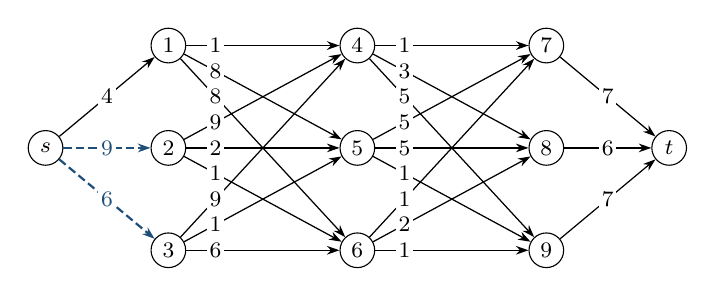
\begin{tikzpicture}[
  font=\footnotesize,
  vertex/.style={circle, draw=black, line width=0.4pt, fill=white, inner sep=0pt, minimum size=4.4mm},
  arc/.style={draw=black, line width=0.45pt, -{Stealth[length=1.6mm, width=1.1mm]}},
  removed/.style={arc, draw=qaccent, line width=0.8pt, dash pattern=on 3pt off 1.5pt},
  capacity/.style={fill=white, inner sep=1pt},
]
\node[vertex] (s) at (0.840,1.300) {$s$};
\node[vertex] (v1) at (2.400,2.600) {1};
\node[vertex] (v2) at (2.400,1.300) {2};
\node[vertex] (v3) at (2.400,0.000) {3};
\node[vertex] (v4) at (4.800,2.600) {4};
\node[vertex] (v5) at (4.800,1.300) {5};
\node[vertex] (v6) at (4.800,0.000) {6};
\node[vertex] (v7) at (7.200,2.600) {7};
\node[vertex] (v8) at (7.200,1.300) {8};
\node[vertex] (v9) at (7.200,0.000) {9};
\node[vertex] (t) at (8.760,1.300) {$t$};
\draw[arc] (s) -- (v1);
\draw[removed] (s) -- (v2);
\draw[removed] (s) -- (v3);
\draw[arc] (v1) -- (v4);
\draw[arc] (v1) -- (v5);
\draw[arc] (v1) -- (v6);
\draw[arc] (v2) -- (v4);
\draw[arc] (v2) -- (v5);
\draw[arc] (v2) -- (v6);
\draw[arc] (v3) -- (v4);
\draw[arc] (v3) -- (v5);
\draw[arc] (v3) -- (v6);
\draw[arc] (v4) -- (v7);
\draw[arc] (v4) -- (v8);
\draw[arc] (v4) -- (v9);
\draw[arc] (v5) -- (v7);
\draw[arc] (v5) -- (v8);
\draw[arc] (v5) -- (v9);
\draw[arc] (v6) -- (v7);
\draw[arc] (v6) -- (v8);
\draw[arc] (v6) -- (v9);
\draw[arc] (v7) -- (t);
\draw[arc] (v8) -- (t);
\draw[arc] (v9) -- (t);
\node[capacity] at (1.620,1.950) {4};
\node[capacity, text=qaccent] at (1.620,1.300) {9};
\node[capacity, text=qaccent] at (1.620,0.650) {6};
\node[capacity] at (3.000,2.600) {1};
\node[capacity] at (3.000,2.275) {8};
\node[capacity] at (3.000,1.950) {8};
\node[capacity] at (3.000,1.625) {9};
\node[capacity] at (3.000,1.300) {2};
\node[capacity] at (3.000,0.975) {1};
\node[capacity] at (3.000,0.650) {9};
\node[capacity] at (3.000,0.325) {1};
\node[capacity] at (3.000,0.000) {6};
\node[capacity] at (5.400,2.600) {1};
\node[capacity] at (5.400,2.275) {3};
\node[capacity] at (5.400,1.950) {5};
\node[capacity] at (5.400,1.625) {5};
\node[capacity] at (5.400,1.300) {5};
\node[capacity] at (5.400,0.975) {1};
\node[capacity] at (5.400,0.650) {1};
\node[capacity] at (5.400,0.325) {2};
\node[capacity] at (5.400,0.000) {1};
\node[capacity] at (7.980,1.950) {7};
\node[capacity] at (7.980,1.300) {6};
\node[capacity] at (7.980,0.650) {7};
\end{tikzpicture}

\caption{Layered instance with $w=3$ ($n=11$, $m=24$, unit costs, $k=2$, $N=301$) and arc capacities. The dashed arcs form the only optimal plan, which reduces the maximum flow from $F(0)=19$ to $\Fstar=4$.}\label{fig:example}
\end{figure}

Experiment E1 measures how the cost to the optimum scales on 30 layered instances (H1). Experiment E2 counts the resources of the interface on nine random instances with 3 to 14 arcs. Experiment E3 runs amplitude amplification on hardware (H2). Its instance is the first seed of the random family with $n=3$ and $m=3$ whose instance has $k=1<\kappa$, a single optimal plan ($M=1$), and $0<\Fstar<F(0)$, which we selected automatically. Both E3 variants use the same truth-table oracle, which marks only the optimal plan (threshold $\tau=\Fstar+1$). The \emph{interface} variant uses the Dicke preparation over $\mathcal{F}_1$ ($N=4$). The \emph{hypercube} variant uses $H^{\otimes 3}$ ($N=8$) and enforces the budget only implicitly through the oracle. We accessed IBM processors through the Open Plan of the IBM Quantum Platform, which offered a monthly quota of 10 minutes of processor time when this paper was written. The eight circuits of E3 formed a single job that used a few seconds of this quota. The MILP scaling study solved random and layered instances with general costs to find the largest networks for which the MILP certifies the optimum within 20 seconds.

\subsection{Methods}\label{sec:method-methods}

\paragraph{Minimum finding at the query level.} The quantum algorithm is Algorithm~\ref{alg:dh}. Simulating it does not require simulating the oracle gate by gate. For each instance, we enumerate $\Fk$ once and compute $F(x)$ for every plan with a classical maximum flow routine, and this table defines the oracle. This is valid because we measure the number of queries and evaluations rather than the time of each one. Given a threshold $\tau$ and $j$ iterations, the outcome is drawn from the exact distribution of amplitude amplification from $\Ak$. With probability $\sin^2((2j+1)\theta)$, where $\sin^2\theta=M_\tau/N$, the outcome is a marked plan chosen uniformly among the marked ones, and otherwise it is an unmarked plan chosen uniformly (Section~\ref{sec:bg-grover}). This \emph{reduced} simulator draws each outcome in $\bigO(\log N)$ time after sorting the flows, which makes $N\approx 10^6$ reachable. We validated it against a \emph{state-vector} simulator that stores the $N$ amplitudes and applies the oracle and the reflection explicitly (Section~\ref{sec:method-validation}). In E1, each run stops at the first measurement of an optimal plan, and we record the queries and evaluations up to that point and whether their sum fits within the budget $Q$ of Proposition~\ref{prop:advantage}. Because the random choices of a run do not depend on when the run is interrupted, this record is exactly the success indicator of a run interrupted at $Q$.

\paragraph{Classical rivals.} Exhaustive enumeration evaluates every plan of $\Fk$, first by cardinality and then in lexicographic order, and certifies the optimum with exactly $N$ evaluations. Random-order search evaluates the plans of $\Fk$ in uniformly random order until it finds an optimal plan. It has the same kind of probabilistic guarantee as the quantum algorithm, and its expected cost is $(N+1)/(M+1)$ evaluations. Both rivals search the same set $\Fk$ as the quantum algorithm.

\paragraph{Reference optimum.} For each instance, we solve the MILP~\eqref{eq:milp} with HiGHS~\cite{highs2018} through SciPy~\cite{scipy2020}, which certifies $\Fstar$ independently of the enumeration. Every solution returned by any method is re-evaluated by an independent maximum flow computation before it is counted.

\paragraph{Circuits.} We implemented the preparation $\Ak$, the truth-table oracle, the arithmetic oracle, and the Grover iteration (built with \texttt{grover\_operator}) in Qiskit~\cite{qiskit2024}. Logical resources are counted after transpilation to the basis $\{\texttt{cx},\texttt{u}\}$ without connectivity constraints, and physical resources after transpilation to \texttt{FakeFez}, the noise model of the 156-qubit IBM Heron processor \texttt{ibm\_fez}. The circuits run with the \texttt{SamplerV2} primitive of Qiskit IBM Runtime on the ideal Aer simulator, on \texttt{FakeFez}, and on the IBM processor.

\subsection{Metrics}\label{sec:method-metrics}
\begin{itemize}
\item The \emph{cost to the optimum} is the number of queries plus evaluations until an optimal plan is first measured (minimum finding), the number of evaluations until an optimal plan is found (random-order search), or $N$ (enumeration). For each instance, we use the mean over the $R$ runs.
\item The \emph{scaling exponent} $\beta$ is the least-squares slope of $\log_{10}$ of the mean cost against $\log_{10}N$ over the 30 instances. We also fit it against $\log_{10}(N/M)$ to separate the effect of the number of optimal plans, and we obtain 95\% confidence intervals from 2{,}000 bootstrap resamples of the instances. We fit no exponent for enumeration, whose cost is $N$ by definition.
\item \emph{Success within the theoretical budget} is the fraction of runs whose cost to the optimum is at most $Q$, which Proposition~\ref{prop:advantage} guarantees to be at least $1/2$.
\item \emph{Resources} are the number of qubits, the number of two-qubit gates, and the circuit depth, in logical and transpiled form.
\item \emph{Amplification} is the frequency of the optimal plan among the shots. We compare it with the uniform baseline $1/N$ using a one-sided binomial test, with the theoretical probability $\sin^2((2j+1)\theta)$ using the ratio of the two and a 95\% Wilson interval, and with the frequency on \texttt{FakeFez} using a two-sided Fisher exact test. For the hardware job, we also record the processor time reported by IBM and the wall-clock time from submission to result, which includes the queue.
\item The \emph{classical context} consists of the wall-clock time of the MILP and of single-threaded enumeration of $\Fk$ on the instances of E1, and of the largest network size up to which the MILP certified all three seeds of every size in the MILP scaling study.
\end{itemize}

\subsection{Hypotheses and refutation criteria}\label{sec:method-hypotheses}
\paragraph{H1 (scaling in simulation).} H1 is refuted if the fitted exponent $\beta$ of minimum finding falls outside $[0.4,0.6]$. The decision uses the point estimate, and we report the confidence interval. Because the reduced simulator draws each outcome from the exact amplification probability, an exponent close to $0.5$ follows from the theory under test whenever the control loop and the cost accounting are implemented correctly. H1 is therefore a correctness check of the implementation, not a test of a physical oracle. The registered interval is also wide for a theoretical value of $0.5$, so we additionally report whether the confidence interval contains $0.5$, a check that was not part of the registered criterion.

\paragraph{H2 (hardware).} On an IBM processor, after the optimal number of iterations of each variant ($j=1$ for the interface variant, where theory gives probability one, and $j=2$ for the hypercube variant, where it gives $0.945$), the frequency of the optimal plan is significantly greater than $1/N$ (one-sided binomial test at level $0.05$). H2 is refuted otherwise. This registered baseline is weak, because any circuit that works at all should pass it. We therefore also compare the hardware frequency with the theoretical probability and with the frequency on \texttt{FakeFez}. We defined these comparisons after the hardware run, so we report them as exploratory and not as tests of a hypothesis fixed in advance.

\subsection{Validation before measurement}\label{sec:method-validation}
No number of E1 was produced before the following checks, implemented as automated tests in the repository, had passed.
\begin{enumerate}
\item The reduced and state-vector simulators give the same outcome distribution, up to $10^{-10}$, for every threshold and for $0$ to $2\sqrt{N}+1$ iterations, with $N\le 2^{10}$.
\item The Qiskit preparation $\Ak$ produces the uniform superposition over $\Fk$ for all $m\le 6$ and $0\le k\le m$, and the Qiskit Grover circuit reproduces the distribution of the query-level model up to $10^{-10}$ for $0$ to $3$ iterations, which links the circuits to the simulator used in E1.
\item The arithmetic oracle flips the sign of exactly the pairs $(x,\alpha)$ with $C(\alpha,x)<\tau$ on all $2^{7}$ basis states of an instance with five arcs and returns every ancilla to zero.
\end{enumerate}
The last check exposed an error in the first version of our arithmetic oracle, in which the circuit synthesizer treated input qubits that had not yet been acted on as clean ancillas. We rebuilt the oracle with an explicit work register before counting any resources. For the hardware experiment, each circuit first ran on the ideal simulator and was accepted only if every frequency of the optimum lay within three standard errors of theory. It then ran on the noisy simulator and only afterwards on the processor.

\subsection{Computational environment}
All classical computations ran on a laptop with an Intel Core i5-1335U processor and 14.8\,GB of memory, using Python 3.14.4, Qiskit 2.6.1, Qiskit Aer 0.18.2, and Qiskit IBM Runtime 0.51.0. Wall-clock times were measured on a single thread, except for the MILP, for which HiGHS chooses the number of threads.

\subsection{Code and data availability}\label{sec:method-code}
The code, the experiment records, and the notebooks that produce every figure and table are publicly available at \url{https://github.com/VinTesta/q-mfnip}. The code is a Python package with a locked environment (\texttt{uv.lock}), and every number in Section~\ref{sec:results} is read from files written by the notebooks. The repository contains the package (\texttt{src/qmfnip/}), the validation tests of Section~\ref{sec:method-validation} (\texttt{tests/}), one notebook per experiment (\texttt{notebooks/}), and one output folder per experiment with its manifest, environment, instances, run records, summaries, and the identifier of the hardware job (\texttt{outputs/}). It also contains the experimental protocol, the list of reported results with the file each number comes from, and the queries of the literature search (\texttt{docs/}).

\section{Results}\label{sec:results}

\subsection{Validation}\label{sec:results-validation}
All checks of Section~\ref{sec:method-validation} passed before the measurements. The MILP certified the optimum of all 30 instances of E1, the optimum over the enumerated space $\Fk$ matched the MILP on all 30, and all instances were non-degenerate ($0<\Fstar<F(0)$). An independent maximum flow computation confirmed the optimality of each of the 18{,}000 runs that reported an optimal plan.

\subsection{Scaling of the cost to the optimum (H1)}\label{sec:results-scaling}
The mean cost of minimum finding grew with the square root of the number of feasible plans, and that of random-order search grew linearly (Fig.~\ref{fig:scaling}). Against $N$, the fitted exponent of minimum finding was $\beta=0.494$ (95\% CI $[0.460,0.523]$, $R^2=0.977$), inside the registered interval $[0.4,0.6]$, so H1 is not refuted. The confidence interval also contains the theoretical value $0.5$. Random-order search had $\beta=0.975$ ($[0.940,1.006]$). Against $N/M$, which accounts for the number of optimal plans, the exponents were $0.510$ ($[0.497,0.529]$, $R^2=0.995$) and $1.001$ ($[0.984,1.022]$), respectively.

On the three largest instances ($N=974{,}121$), minimum finding reached the optimum after 1{,}750 queries and evaluations on average, against 383{,}687 evaluations for random-order search and 974{,}121 for enumeration. Across instances, the mean cost of minimum finding ranged from $0.90\sqrt{N}$ to $2.67\sqrt{N}$, and the lowest values occurred on instances with several optimal plans ($M$ up to 4). All 6{,}000 runs of minimum finding reached the optimum within the budget $Q$ of Proposition~\ref{prop:advantage}, counting queries and evaluations, and the mean cost never exceeded 10.1\% of $Q$. Averaged over the instances, the mean cost of random-order search was within 1\% of the theoretical value $(N+1)/(M+1)$.

\begin{figure}[t]
\centering
\begin{tikzpicture}[font=\footnotesize]
\begin{loglogaxis}[
  width=\linewidth,
  height=5.3cm,
  xmin=5, xmax=2.5e6,
  ymin=1, ymax=2.5e6,
  xtickten={1,...,6},
  ytickten={0,...,6},
  xminorticks=false,
  yminorticks=false,
  tick pos=left,
  tick align=outside,
  major tick length=2.5pt,
  xlabel={Number of feasible plans $N$},
  ylabel={Mean cost to the optimum},
  label style={font=\footnotesize},
  tick label style={font=\footnotesize},
  axis line style={line width=0.4pt},
  every tick/.style={black, line width=0.4pt},
  table/col sep=comma,
]
\addplot[qgray, line width=0.6pt, dotted] table[x=N, y=N] {figures/data/scaling_fits.csv}
  node[pos=1, anchor=west, text=qgray] {$N$};
\addplot[black, line width=0.6pt] table[x=N, y=random_order] {figures/data/scaling_fits.csv}
  node[pos=0.8, sloped, anchor=north, yshift=-2pt] {random-order search};
\addplot[qaccent, line width=0.6pt] table[x=N, y=durr_hoyer] {figures/data/scaling_fits.csv}
  node[pos=0.8, sloped, anchor=north, yshift=-3pt, text=qaccent] {minimum finding};
\addplot[only marks, mark=square, mark size=1.2pt, mark options={black, line width=0.5pt, fill=white}] table[x=N, y=random_order] {figures/data/scaling_points.csv};
\addplot[only marks, mark=*, mark size=1.2pt, mark options={qaccent, line width=0.5pt, fill=qaccent}] table[x=N, y=durr_hoyer] {figures/data/scaling_points.csv};
\end{loglogaxis}
\end{tikzpicture}

\caption{Mean cost to the optimum of minimum finding and random-order search on the 30 instances of E1 (200 runs per instance), with least-squares fits and the enumeration cost $N$ for reference.}\label{fig:scaling}
\end{figure}

\subsection{Resources of the interface}\label{sec:results-resources}
The Dicke preparation was the cheapest component and the arithmetic oracle the most expensive (Table~\ref{tab:resources}). For networks with 3 to 14 arcs, the preparation $\Ak$ used 8 to 174 two-qubit gates in the logical count. The truth-table oracle grew quickly with $m$ and with the number of marked plans. The arithmetic oracle over $(x,\alpha)$ used 18 to 46 qubits, of which only $m+n-2$ take part in the search, while the others are ancillas for the cut indicators, the weighted sum, and the comparison. It needed 690 to 4{,}202 two-qubit gates in the logical count and 2{,}055 to 14{,}296 after transpilation to the Heron model, where routing on the heavy-hex connectivity roughly triples the count. The condition $2^{n-2}<N$ held on 7 of the 9 instances and failed on the two instances with $k=1$ and $n\ge 6$.

\begin{table*}[t]
\centering
\caption{Two-qubit gate counts of the interface components on the instances of E2, logical (basis \texttt{cx}, \texttt{u}) / transpiled for \texttt{FakeFez} at optimization level 1. The truth-table oracle marks the $M$ optimal plans, and the last column states whether $2^{n-2}<N$.}\label{tab:resources}
\small
\begin{tabular}{rrrrrrrrc}
\toprule
$n$ & $m$ & $k$ & $N$ & $A_k$ & Truth table & Arith. qubits & Arith. oracle & $2^{n-2}<N$ \\
\midrule
3 & 3 & 1 & 4 & 8 / 8 & 6 / 9 & 18 & 690 / 2{,}055 & yes \\
4 & 7 & 1 & 8 & 24 / 24 & 122 / 242 & 29 & 2{,}008 / 6{,}533 & yes \\
4 & 7 & 2 & 29 & 76 / 121 & 122 / 242 & 29 & 2{,}014 / 6{,}353 & yes \\
5 & 10 & 1 & 11 & 36 / 36 & 290 / 686 & 34 & 2{,}344 / 7{,}465 & yes \\
5 & 10 & 2 & 56 & 118 / 190 & 290 / 686 & 34 & 2{,}338 / 7{,}315 & yes \\
6 & 12 & 1 & 13 & 44 / 44 & 442 / 1{,}096 & 43 & 4{,}202 / 14{,}296 & no \\
6 & 12 & 2 & 79 & 146 / 236 & 442 / 1{,}096 & 43 & 4{,}202 / 14{,}296 & yes \\
7 & 14 & 1 & 15 & 52 / 52 & 1{,}252 / 3{,}058 & 46 & 4{,}140 / 13{,}615 & no \\
7 & 14 & 2 & 106 & 174 / 282 & 626 / 1{,}514 & 46 & 4{,}146 / 13{,}927 & yes \\
\bottomrule
\end{tabular}
\end{table*}


\subsection{Amplitude amplification on quantum hardware (H2)}\label{sec:results-hardware}
The E3 instance has three arcs, $s\to 1$, $s\to t$, and $1\to t$, with capacities 7, 10, and 6, maximum flow $F(0)=16$, and a single optimal plan, which removes $s\to t$ and leaves $\Fstar=6$. On the ideal simulator, the frequency of the optimal plan was within three standard errors of theory in all eight circuits. Table~\ref{tab:hardware} lists the frequencies at the optimal number of iterations. On the IBM Heron processor \texttt{ibm\_fez} (job \texttt{dbmujid8mdtc73d8m2h0}), the optimal plan was measured with frequency $0.815$ in the interface variant after one iteration and $0.818$ in the hypercube variant after two, well above the baselines $1/4$ and $1/8$ (one-sided binomial test, $p<10^{-300}$ in both cases), so H2 is not refuted. The noise model \texttt{FakeFez} gave $0.898$ and $0.833$ for the same circuits.

In the exploratory comparison, the hardware frequency in the interface variant (95\% Wilson interval $[0.803,0.827]$) reached 81.5\% of the theoretical probability of one and was significantly lower than on \texttt{FakeFez} (difference $0.083$, two-sided Fisher exact test, $p<10^{-26}$). In the hypercube variant, the hardware frequency ($[0.806,0.829]$) reached 86.5\% of the theoretical probability of $0.945$ and did not differ significantly from \texttt{FakeFez} (difference $0.016$, $p=0.06$). With the interface preparation, the frequency of the optimum dropped back to $0.215$ and $0.233$ after two and three iterations, close to the theoretical value of $0.25$. In the interface variant, the fraction of shots inside $\mathcal{F}_1$ fell from $0.983$ without iterations to $0.917$ after one iteration and $0.880$ after three. The job waited 41.2 minutes in the queue of the free plan and used 11 seconds of processor time.

\begin{table*}[t]
\centering
\caption{Frequency of the optimal plan at the optimal number of Grover iterations $j$ for the E3 instance (4{,}096 shots per circuit), with circuit depth and two-qubit gates after transpilation and the one-sided binomial $p$-value against $1/N$.}\label{tab:hardware}
\small
\begin{tabular}{llrrrrrrr}
\toprule
Environment & Variant & $j$ & Depth & 2q gates & Theory & Frequency & $1/N$ & $p$ \\
\midrule
ideal simulator & interface & 1 & -- & -- & 1.000 & 1.000 & 0.250 & $<10^{-300}$ \\
ideal simulator & hypercube & 2 & -- & -- & 0.945 & 0.942 & 0.125 & $<10^{-300}$ \\
noise model (\texttt{FakeFez}) & interface & 1 & 110 & 29 & 1.000 & 0.898 & 0.250 & $<10^{-300}$ \\
noise model (\texttt{FakeFez}) & hypercube & 2 & 144 & 39 & 0.945 & 0.833 & 0.125 & $<10^{-300}$ \\
hardware (\texttt{ibm\_fez}) & interface & 1 & 110 & 29 & 1.000 & 0.815 & 0.250 & $<10^{-300}$ \\
hardware (\texttt{ibm\_fez}) & hypercube & 2 & 144 & 39 & 0.945 & 0.818 & 0.125 & $<10^{-300}$ \\
\bottomrule
\end{tabular}
\end{table*}


\subsection{Classical context}\label{sec:results-classical}
The MILP solved every instance of E1 in at most 24\,ms, with no visible growth with $N$, whereas single-threaded enumeration of $\Fk$ grew linearly with $N$ and took up to 568\,s on the largest instances. In the MILP scaling study, with general costs and a limit of 20\,s, the MILP certified all three seeds of every size up to 2{,}560 nodes and 7{,}680 arcs in the random family with budgets of 50\% and 75\% of the cheapest cut. In the layered family it certified all seeds up to 4{,}098 nodes and 12{,}224 arcs, the largest size tested, with the same budgets. With a budget of 25\%, the corresponding sizes were 320 nodes in the random family, where one instance with 640 nodes exceeded the limit, and 2{,}306 nodes in the layered family.

\section{Discussion and Limitations}\label{sec:discussion}

\paragraph{Which rival the speedup beats} Proposition~\ref{prop:advantage} compares the quantum interface with classical algorithms that learn about the network only by evaluating the flow of candidate plans. Exhaustive enumeration of $\Fk$ is the best algorithm of this kind up to a factor of two, and the simulations confirm the separation that the proposition predicts (Section~\ref{sec:results-scaling}). The comparison says nothing about algorithms that exploit the structure of the network, and the MILP is one of them. On the instances of E1 it was several orders of magnitude faster than both searches (Section~\ref{sec:results-classical}), so the query-level speedup holds only relative to exhaustive search.

\paragraph{When the speedup matters} When $k$ grows with the network, the quantum algorithm still needs $\Theta(\sqrt{N})$ oracle calls, which is exponential in $k$. Proposition~\ref{prop:advantage} is thus a quadratic speedup over exhaustive search and not an efficient algorithm for an NP-hard problem.

\paragraph{Cost of the oracle} The proposition counts oracle calls of polynomial size, but the polynomial matters. The arithmetic realization of Section~\ref{sec:interface-oracle}, the only one we built for general instances, already needs hundreds to thousands of two-qubit gates on networks with at most 14 arcs (Table~\ref{tab:resources}). It also searches the larger space of pairs $(x,\alpha)$ and can beat enumeration of $\Fk$ in query count only when $2^{n-2}<N$, which held on 7 of the 9 instances of E2. A reversible maximum flow circuit, which the speedup over $\Fk$ requires, would be larger still, and Proposition~\ref{prop:advantage} currently relies on an existence argument for it rather than on an explicit construction. Babbush \emph{et al.}~\cite{babbush2021} estimate that quadratic speedups need very long runs to offset the overhead of error correction on early fault-tolerant hardware. For the MFNIP, where every query contains a maximum flow computation, the crossover with classical enumeration would appear only for very large $N$, and the crossover with the MILP may never occur.

\paragraph{General costs} The interface depends on a uniform superposition of the feasible plans. With unit costs, Dicke states provide this superposition. With arbitrary integer costs, it becomes a uniform superposition over the solutions of a knapsack constraint, for which we know no efficient preparation. The provable speedup therefore holds only for the cardinality variant.

\paragraph{What the hardware experiment shows} The truth-table oracle used on the processor marks a plan found beforehand by classical means, and its cost grows exponentially with $m$. The experiment shows that the interface, consisting of the preparation, the oracle, and the reflection, amplifies the optimal plan on a three-arc instance. It does not demonstrate a speedup and would not scale. At the optimal number of iterations, the transpiled interface circuit had fewer two-qubit gates than the hypercube circuit (29 against 39) and a higher frequency of the optimum on the noise model (0.898 against 0.833). On the processor, however, the two frequencies were practically equal (0.815 and 0.818, Table~\ref{tab:hardware}), so the higher ideal probability of the interface variant did not carry over to the hardware. The noise model predicted the hypercube circuit well but overestimated the interface circuit. Because we defined these comparisons after the run, a new hardware run with the comparison against the noise model registered in advance is needed to confirm them. Noise also produced plans outside the budget, which the classical loop must discard after evaluating them.

\paragraph{Threats to validity} The scaling experiment simulates the algorithm at the query level, so it verifies the query complexity of the interface and the correctness of the control loop but not the behavior of a physical oracle. The link between the simulator and the circuits was verified only on small instances (Section~\ref{sec:method-validation}). The instances come from two synthetic generators and are small. The layered family has a fixed number of arcs for each width, so $N$ grows together with $k$ and $m$. The number of optimal plans $M$ also varies across instances, which is why we also fit against $N/M$. Finally, the literature search covered titles and abstracts in four sources and may have missed work indexed elsewhere.

\section{Conclusion and Future Work}\label{sec:conclusion}

We proposed a quantum interface that applies quantum minimum finding to the maximum flow network interdiction problem. It uses one qubit per arc, a Dicke-state preparation that enforces a cardinality budget, and a phase oracle that compares the follower's maximum flow with a threshold. With this interface, the quantum algorithm searches the same set of feasible plans as classical exhaustive enumeration and needs quadratically fewer accesses to the objective function, which is optimal in the query model (Proposition~\ref{prop:advantage}). Simulations on 30 instances agreed with the predicted square-root growth. We counted the gates of the interface components and ran amplitude amplification for a three-arc instance on an IBM processor, where the optimal plan appeared in 81.5\% of the shots against 25\% under uniform sampling. The speedup holds relative to exhaustive search, and the MILP remained much faster on every instance we could simulate.

Future work follows from these limitations. (i) A quantum speedup for branch-and-bound~\cite{montanaro2020} applied to the MILP would allow a comparison with the method used in practice. (ii) An explicit reversible maximum flow oracle with gate counts would replace the existence argument in Proposition~\ref{prop:advantage}. (iii) Resource estimates in the fault-tolerant regime would locate the crossover with classical enumeration and with the MILP. (iv) Efficient state preparations for general interdiction costs would extend the speedup beyond the cardinality variant. (v) A hardware run with the comparison against the noise model registered in advance would turn the exploratory analysis of Section~\ref{sec:results-hardware} into a test.


\bibliographystyle{IEEEtran}
\bibliography{references}
\end{document}
